% ============================================================================
\section{Multimodal detection on wearable data (SeizeIT2)}
\label{sec:seizeit2}

\subsection{Dataset}

SeizeIT2 (Bhagubai et al.\ 2025; OpenNeuro ds005873 v1.1.0, CC0) was recorded with the Byteflies Sensor Dot in five European epilepsy monitoring units (Leuven, Freiburg, Aachen, Karolinska, Coimbra). It is almost exactly the ear-hook's sensor set.

\begin{table}[H]
\centering\small
\caption{SeizeIT2 as used here.}
\begin{tabularx}{\linewidth}{@{}l L@{}}
\toprule
Patients & 125 with focal epilepsy (51 female; children only from Leuven) \\
Seizures & 883 focal (aware, impaired awareness, focal-to-bilateral tonic-clonic, unclear); mean 58 s (3 s -- 16 min) \\
Recording & 11,626 h in 2,850 runs \\
EEG & 2 behind-the-ear (mastoid) channels, 256 Hz: a same-side channel and a cross-head channel (or two lateral channels in a ``generalized'' montage); montage left/right/generalized in 65/44/16 patients \\
ECG, EMG & 1 chest ECG channel and 1 left-deltoid EMG channel, 256 Hz \\
Motion & Accelerometer and gyroscope on two devices (upper back, chest), 25 Hz \\
Missing & ECG/EMG absent in 46 runs, motion in 299 runs \\
Labels & Clinician-marked onset/offset from video-EEG; type, lateralization, localization, vigilance; ``bckg'' background and ``impd'' epochs \\
\bottomrule
\end{tabularx}
\end{table}

\subsection{Streaming 126 GB through memory}

The dataset is 126\,GB and the laptop had 19\,GB free. The user asked whether training could use the data online without compromising quality: streaming reads exactly the same samples a download would, so it loses no quality. For each run the four EDF files were fetched in parallel from S3 into RAM, decoded by a small built-in EDF reader (header fields: labels, physical and digital ranges, samples per record; int16 data scaled to physical units, EDF-Annotations channel skipped), converted to features, and only the features were saved atomically (1.8\,GB total). Three runs streamed in parallel over 12 connections at 18--25\,MB/s; the job was resumable. The file listing was obtained from the S3 API (2,850 event files downloaded in parallel).

\subsection{Features}

Signals were cut into 4\,s windows every 2\,s (enough heartbeats for HR; manageable for 11,600\,h); a window is ``seizure'' if its centre lies in a marked seizure.

\begin{itemize}
\item \textbf{EEG (2 ch, 28 features):} band-pass 0.5--45\,Hz; per channel line length, log variance, Hjorth mobility and complexity, five log band powers and five relative band powers (Hann-windowed FFT), identical to the CHB-MIT features.
\item \textbf{ECG (8):} R-peaks by a Pan--Tompkins-style detector (5--20\,Hz band-pass, squared derivative, 120\,ms moving average, adaptive threshold at 30\% of the 98th percentile per 10\,s block, 270\,ms refractory), RR intervals kept if 0.27--2.0\,s and within 30\% of a 9-beat running median; features HR over 4, 10 and 30\,s, 30\,s HR rise, RMSSD and SDNN over 30\,s, beat quality (beats found vs expected) and ECG line length.
\item \textbf{EMG (5):} 20--120\,Hz band-pass with a 48--52\,Hz notch; log RMS, line length, zero-crossing rate, fraction of power above 60\,Hz, and 0.5--20\,Hz log power.
\item \textbf{Motion (8):} per device, log standard deviation and line length of acceleration magnitude, fraction of power at 2--8\,Hz (clonic band) and mean gyroscope magnitude.
\end{itemize}

Every feature is z-scored against a causal exponential moving average of the previous $\approx$10\,min of the same recording (EMA over 300 two-second windows); absolute HR and beat quality are also kept. Missing sensors stay NaN and are routed separately by the trees, so no patient is dropped.

\subsection{Models and evaluation}

HistGradientBoosting (150 trees, class-balanced) trained on all seizure windows plus 3\% of others; patient-wise 5-fold cross-validation balanced by seizure count (every patient scored by a model that never saw them); probability smoothed over 3 windows (6\,s), threshold, 60\,s refractory; a seizure is caught if an alarm fires from 15\,s before onset to its end, other alarms are false except within 60\,s after a seizure; thresholds swept from 0.05 to 0.99.

The fair comparison is false alarms at \emph{matched sensitivity}: the fewest false alarms at any threshold catching at least X\%. \textbf{A bug was caught here}: the first summary interpolated false alarms along the sensitivity curve, but sensitivity is not monotonic in the threshold (at low thresholds a false alarm just before a seizure starts the refractory period and blocks the true alarm), which produced nonsense (EEG-only apparently 1,300\,\FAd{} at 60\%); it was replaced by the minimum over thresholds.

Two kinds of numbers are reported. \emph{Calibrated} numbers fix the threshold in advance on tuning data and score later data (what a device would experience). \emph{Best-along-the-curve} numbers sweep the threshold over the test data and report the best point within a budget; they compare setups fairly but are slightly optimistic for deployment. For the one-stage general model the two agree closely (14\%/25\% at $\le$1/$\le$5 per day both ways).

\subsection{Main results (125 patients, 883 seizures)}

\begin{table}[H]
\centering\small
\caption{False alarms per 24 h at matched sensitivity (lower is better).}
\label{tab:sz2main}
\begin{tabular}{@{}lcccc@{}}
\toprule
Setup & 50\% caught & 60\% & 70\% & 80\% \\
\midrule
EEG only (ear) & 103.7 & 161.7 & 294.4 & not reached \\
ECG only & 132.6 & 225.6 & 378.2 & 677.8 \\
Body only (ECG+EMG+motion) & 116.3 & 193.5 & 283.8 & 583.1 \\
\textbf{EEG + ECG} & \textbf{85.5} ($-18$\%) & \textbf{122.8} ($-24$\%) & \textbf{204.0} ($-31$\%) & \textbf{459.2} \\
EEG + ECG + EMG + motion & 75.4 ($-27$\%) & 139.3 ($-14$\%) & 211.7 ($-28$\%) & 539.9 \\
\bottomrule
\end{tabular}
\end{table}

\begin{table}[H]
\centering\small
\caption{Seizures caught within a daily false-alarm budget, and at the default threshold 0.5.}
\begin{tabular}{@{}lccccc|ccc@{}}
\toprule
Setup & $\le$5 & $\le$20 & $\le$50 & $\le$100 & $\le$200 & Caught @0.5 & FA/day & Latency \\
\midrule
EEG only & 14\% & 23\% & 23\% & 42\% & 62\% & 79.4\% & 608 & 6 s \\
ECG only & 16\% & 29\% & 29\% & 48\% & 60\% & 74.0\% & 438 & 7 s \\
Body only & 16\% & 28\% & 42\% & 50\% & 64\% & 75.4\% & 386 & 8 s \\
\textbf{EEG + ECG} & \textbf{21\%} & \textbf{35\%} & 35\% & \textbf{57\%} & 66\% & 78.7\% & \textbf{399} & 7 s \\
All four & 20\% & 34\% & \textbf{45\%} & 53\% & \textbf{68\%} & 78.3\% & 348 & 7 s \\
\bottomrule
\end{tabular}
\end{table}

Per patient, the median false-alarm rate fell from 618 (IQR 533--686) with EEG to 373 (329--440) with EEG + ECG and 342 (299--400) with all four; EEG + ECG had fewer false alarms than EEG alone in \textbf{115/125} patients (all four: 120/125), while detections per patient barely changed (more in 16, fewer in 21). Heart rate is the add-on that pays; for focal seizures the heart alone rivals the ear EEG under strict budgets; EMG and motion as direct features give no consistent gain for these mostly non-convulsive seizures. Two interim snapshots taken while streaming (48 patients: $-7$\% to $-20$\%; 78 patients: $-21$\% to $-44$\%) converged to the final $-18$\% to $-31$\%.

\begin{figure}[H]
\centering
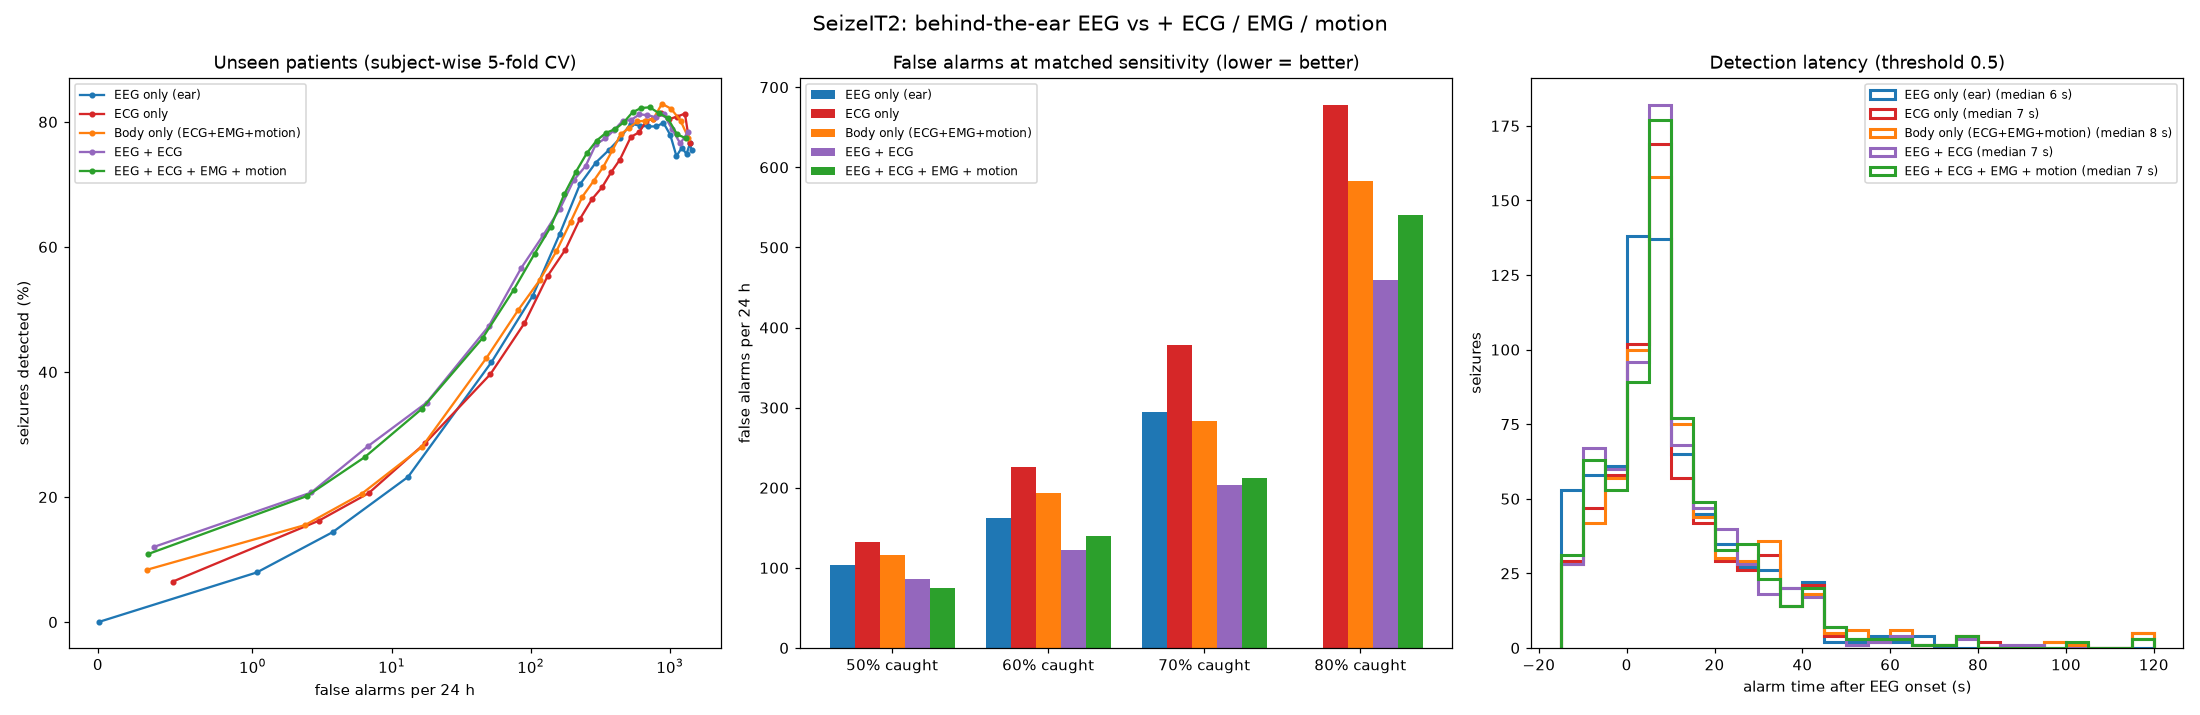
\includegraphics[width=\linewidth]{epilepsy_sim/detect/results_seizeit2/seizeit2.png}
\caption{SeizeIT2: sensitivity vs false alarms, false alarms at matched sensitivity, and latency for all setups (including the later context and HR-excess setups).}
\end{figure}

\subsection{Personal fine-tuning and sustained-alarm rules}

Chronological split per patient: tune on everything up to 10\,min after the $k$-th seizure, test only on later data (71 patients with $k=2$, 649 test seizures; 97 patients with $k=1$, 751). The fine-tuned model adds the patient's tuning windows ($\times$10) to the general model's training data. Three alarm rules were compared: 6\,s smoothing, 10\,s and 20\,s sustained above threshold. A vectorised event scorer was verified identical to the reference scorer on synthetic records before use.

\begin{table}[H]
\centering\small
\caption{Fine-tuning on 2 own seizures (71 patients): FA/day at matched sensitivity and caught within budgets (6 s rule).}
\begin{tabular}{@{}lccccccc@{}}
\toprule
Setup & 40\% & 50\% & 60\% & 70\% & $\le$1/d & $\le$5/d & $\le$20/d \\
\midrule
EEG, general & 100.8 & 157.9 & 221.3 & 289.0 & 0\% & 11\% & 20\% \\
EEG, fine-tuned & 61.5 & 91.6 & 127.9 & 217.1 & 8\% & 15\% & 28\% \\
EEG+ECG, general & 52.4 & 88.7 & 168.0 & 254.7 & 10\% & 18\% & 32\% \\
\textbf{EEG+ECG, fine-tuned} & \textbf{40.5} & \textbf{60.5} & \textbf{107.2} & \textbf{192.5} & \textbf{14\%} & \textbf{21\%} & 27\% \\
\bottomrule
\end{tabular}
\end{table}

ECG ($-44$\% at 50\%) and fine-tuning ($-42$\%) add up ($-62$\% together, close to the $-67$\% expected for independent effects), with unchanged delay. With one tuning seizure, EEG-only tuning was inconsistent (better at 40\%, worse at 60\% and under strict budgets: overfitting to one event), whereas with ECG even one seizure helped ($-16$\% to $-45$\%). Sustained rules helped only at low sensitivity, were worse at 60--70\% caught and added 3--7\,s of delay; 6\,s smoothing was kept.

\subsection{Personal alarm thresholds}

For each budget (0.5--200 \FAd), a personal threshold was the lowest threshold whose false alarms on the patient's own tuning data stayed within budget (fallback to shared for $<$6\,h of tuning data: 12 of 71; median tuning 23\,h); the shared threshold used the same rule on pooled tuning data. Personal thresholds gave no meaningful gain (at most +2--4 points at loose budgets, overshooting their budget, never reaching $\le$1/day): per-person baseline normalisation already puts everyone on a common scale (at 5/day, personal thresholds IQR 0.956--0.971 vs shared 0.971). The general model's shared threshold was \emph{predictable}: budgets of 1/5/20 on tuning data gave 1.4/5.2/20.2 \FAd{} later (EEG+ECG). Fine-tuned models calibrated on their own training data were $\approx$10$\times$ optimistic (0.5--1/day became 10--18/day, later 30--37/day for the richest model); calibration needs held-out data.

\subsection{Why do the false alarms happen?}

All analyses used cached outputs (general model, shared threshold, 71 patients). A \textbf{mistake was caught}: the ``impd'' annotation was first assumed to mean interictal epileptiform discharges; the dataset's \code{events.json} defines it as an \emph{impedance control check} (likely artefactual). Such epochs explained $<$1\% of false alarms (2--5$\times$ chance; 0.19\% of time). False alarms were not hidden seizures (7--10\% within 1--30\,min of a seizure vs 8.9\% of time). They were concentrated: at 5/day the worst 10\% of patients produced 47\% (EEG) and 32\% (EEG+ECG) of them, the worst 25\% 77\% and 59\%; the median patient had 1.4 and 4.0/day. Of 22 patient traits, only \textbf{ear-EEG amplitude instability} (IQR of log-variance) survived Bonferroni correction ($\rho=0.49$, $p=1\times10^{-5}$; 2.10 vs 1.18); no link was found with missing sensors, seizure type, number of seizures, electrode side, sex, recording fragmentation or ECG quality (age is not available). At the moment of a false alarm (EEG+ECG, 3,655 false alarms vs 267 detections) the signals looked like seizures: heart rate 103 vs 110\,bpm (normal 73), a 30\,s HR rise of +20 vs +22, raised movement, EEG power and shoulder EMG: physiological look-alikes (getting up, arousals). EEG-only false alarms instead showed muscle/movement in the EEG (gamma share 0.06$\to$0.13) with a calm heart, which is why ECG removes them. Each patient's tuning-period false-alarm rate predicted their later rate ($\rho$ = 0.56--0.83), flagging 73--81\% of the worst quartile.

\subsection{Long context}

For key features (EEG line length, log variance, $\delta$ and $\theta$ shares; HR, RMSSD, SDNN, beat quality) the model received causal EMAs over 15\,s, 1\,min and 5\,min, fast-minus-slow differences, the 1-min running maximum, and heart features against a 30-min baseline, each context setup training on exactly the same windows as its twin (shared random seed). Causality was verified by altering future data and checking that past features were unchanged.

\begin{table}[H]
\centering\small
\caption{Context and HR-excess setups (125 patients, general model).}
\label{tab:ctx}
\begin{tabular}{@{}lccccccc@{}}
\toprule
Setup & 50\% & 60\% & 70\% & 80\% & $\le$5/d & $\le$50/d & $\le$200/d \\
\midrule
Ear EEG only & 103.7 & 161.7 & 294.4 & -- & 14\% & 23\% & 62\% \\
EEG + context & 72.2 & 148.2 & 287.7 & 770.6 & 21\% & 48\% & 65\% \\
EEG + ECG & 85.5 & 122.8 & 204.0 & 459.2 & 21\% & 35\% & 66\% \\
EEG + ECG + context & 59.5 & 98.5 & 194.6 & 401.8 & 25\% & 48\% & 72\% \\
EEG + ECG + HR-excess & 49.2 & 111.7 & 177.7 & 385.8 & 20\% & 50\% & 72\% \\
\textbf{EEG + ECG + context + HR-excess} & \textbf{39.6} & \textbf{92.5} & \textbf{154.9} & \textbf{368.0} & \textbf{28\%} & \textbf{50\%} & \textbf{73\%} \\
same, big model (\S\ref{sec:big}) & 48.2 & 82.8 & 165.0 & 500.6 & 25\% & 54\% & 72\% \\
EEG + PPG(sim) + context + HR-excess & 44.8 & 83.5 & 175.2 & 376.5 & 26\% & 53\% & -- \\
\bottomrule
\end{tabular}
\end{table}

\subsection{Heart rate not explained by movement (HR-excess)}

Per recording, a causal running linear fit of heart rate on activity predicts the heart rate the current movement explains. With $A_t$ the 15\,s EMA of the larger of the two log-acceleration features and $H_t$ the 10\,s heart rate, running EMAs with 30\,min memory of $A$, $H$, $A^2$ and $AH$ (using only past values) give
\begin{equation}
b_t = \mathrm{clip}\!\left(\frac{\overline{AH}_{t-1}-\bar A_{t-1}\bar H_{t-1}}{\max(\overline{A^2}_{t-1}-\bar A^2_{t-1},0.05)},0,30\right),\qquad
\hat H_t = \bar H_{t-1} + b_t(A_t - \bar A_{t-1}),
\end{equation}
and four features: $H_t-\hat H_t$ (HR excess), its 1\,min EMA, $A_t$, and the 30\,s rise not explained by activity, $(H_t-H_{t-30s}) - b_t(A_t-A_{t-30s})$. A univariate pre-check suggested little value (AUC 0.62 vs 0.61 for raw HR in separating false alarms from detections), yet in the full model HR-excess cut false alarms by 42\% at 50\% caught and, with context, gave the best general model (Table~\ref{tab:ctx}): $-62$/$-43$/$-47$\% at 50/60/70\% caught vs ear EEG alone and 28\% caught at $\le$5/day. \textbf{Lesson: a weak single-feature pre-check does not predict a feature's value in combination.}

\subsection{Benchmarks on SeizeIT2}

\begin{table}[H]
\centering\small
\caption{Published SeizeIT2 results vs ours at similar false-alarm rates (protocols differ; order-of-magnitude comparison).}
\begin{tabularx}{\linewidth}{@{}L l l L@{}}
\toprule
Published & Caught & FA/day & Ours \\
\midrule
Dataset paper, SVM, bte-EEG (29 held-out patients) & 71.1\% & 264 (11.0/h) & EEG only 62\% at $\le$200; EEG+ECG+context 72\% at $\le$200 \\
Dataset paper, ChronoNet & 84.2\% & 2,412 & EEG+ECG+context 80\% at 402 \\
ECG Matrix Profile, FAR-optimised (Reintjes 2025) & 19.6\% & $<$48 & ECG only 29\% at $\le$20 \\
ECG TimeVQVAE-AD, FAR-optimised & 36.9\% & 206 & ECG only 60\% at $\le$200 \\
ECG TimeVQVAE-AD, sensitivity-optimised & 82.8\% & 627 & EEG+ECG+context 80\% at 402 \\
ECG Matrix Profile, responders only & 70.7\% & $\approx$46 & EEG+ECG fine-tuned, responders 81\% at $\le$50 \\
\bottomrule
\end{tabularx}
\end{table}

No published SeizeIT2 result approaches 1 \FAd. The 69\% at 0.49 \FAd{} of Vandecasteele et al.\ (2020) used the earlier SeizeIT1 hospital dataset, a 3-channel setup, patient-specific models and only seizures visible on behind-the-ear EEG; the SeizeIT2 paper calls its own wearable results ``sub par''. Real devices keep false alarms low mainly by targeting convulsive seizures (Embrace, NightWatch), night-only use, personal tuning, user cancellation and better electrodes.

\subsection{Heart responders}

A responder is a patient whose heart rate rose by $>$50\,bpm (max 10\,s HR from onset to 60\,s after end minus the 5-min pre-onset median) in at least one of their first two seizures, a definition a device could apply; 23 of 69 patients with ECG are responders.

\begin{table}[H]
\centering\small
\caption{Responders vs non-responders (71 patients, later data; caught within budgets).}
\begin{tabular}{@{}llccc@{}}
\toprule
Model & Group & $\le$1/day & $\le$5/day & $\le$20/day \\
\midrule
EEG only, general & responders / non-resp. & 10\% / 2\% & 21\% / 7\% & 44\% / 16\% \\
EEG+ECG, general & responders / non-resp. & 25\% / 6\% & 46\% / 10\% & 68\% / 18\% \\
EEG+ECG, fine-tuned & responders / non-resp. & 30\% / 7\% & 50\% / 15\% & 72\% / 24\% \\
Best (ctx+HRx), general & responders / non-resp. & 31\% / 7\% & 55\% / 14\% & 74\% / 23\% \\
Best (ctx+HRx), fine-tuned & responders / non-resp. & \textbf{33\%} / 8\% & \textbf{60\%} / 16\% & \textbf{75\%} / 27\% \\
PPG(sim), fine-tuned & responders / non-resp. & 28\% / 8\% & 54\% / 14\% & 69\% / 26\% \\
\bottomrule
\end{tabular}
\end{table}

\subsection{More data and a bigger model}
\label{sec:big}

With 8\% instead of 3\% of non-seizure windows (the 3\% pool a subset of the 8\% one), 400 trees at learning rate 0.05 and 63 leaves, results were mixed (Table~\ref{tab:ctx}) at 3$\times$ the compute: model capacity and training-set size are not the bottleneck; information is.

\subsection{Two-stage detection and a personal alarm verifier}

Stage 1 (best general model, out-of-fold outputs) raises candidates at 0.5 or 0.7 with a 10\,s candidate refractory. A second HistGradientBoosting model (200 trees, 15 leaves) verifies each candidate at 0 or 10\,s after the trigger using the probability's shape (peak, mean, fraction above 0.8 and 0.95, current value), recent noisiness (candidates in the last 10\,min and hour, 5\,min mean probability) and changes vs the 5\,min before in HR, HR slope, RMSSD, beat quality, EEG log variance, line length, gamma and delta shares, EMG and movement, plus HR-excess features; the 60\,s refractory applies only to accepted alarms. It was trained with patient-wise folds and scored on held-out patients' later data. \textbf{A bug was caught}: the first run grouped alarms per patient although each recording's clock starts at 0, so an alarm in one recording was counted in all others; a debug check (ranking by stage-1 peak lost half the seizures) exposed it and scoring was fixed per recording (``accept all'' then reproduced stage 1: 49\% at 79 \FAd{} on the debug subset). The personal verifier additionally trains on the patient's own tuning-period candidates (weighted $\times$20), which are out-of-sample for stage 1.

\begin{table}[H]
\centering\small
\caption{Two-stage results (candidates at 0.5, decision +10 s; 71 patients, later data).}
\setlength{\tabcolsep}{4pt}
\begin{tabular}{@{}lccccc@{}}
\toprule
Setup & $\le$1/d & $\le$2/d & $\le$5/d & $\le$20/d & $\le$50/d \\
\midrule
One stage (general), all & 14\% & -- & 25\% & 36\% & 47\% \\
Two stage, general verifier, all & 15\% & 18\% & 25\% & 38\% & 54\% \\
Two stage, general + quality features & 14\% & 17\% & 26\% & 39\% & 54\% \\
\textbf{Two stage, personal verifier ($\times$20), all} & \textbf{19\%} & \textbf{22\%} & \textbf{30\%} & \textbf{45\%} & \textbf{60\%} \\
Personal verifier $\times$5 / $\times$50, all & 18\% / 19\% & 22\% / 23\% & 29\% / 30\% & 43\% / 46\% & 57\% / 61\% \\
Personal verifier + quality features, all & 19\% & 23\% & 31\% & 45\% & 61\% \\
\textbf{Personal verifier, responders} & \textbf{39\%} & \textbf{47\%} & \textbf{64\%} & \textbf{77\%} & \textbf{85\%} \\
Personal verifier, non-responders & 11\% & 14\% & 17\% & 32\% & 51\% \\
\bottomrule
\end{tabular}
\end{table}

The personal verifier gave the largest strict-budget gain of anything tried, saturating at weights $\times$20--50. Ear-EEG signal-quality features (5-min log-variance instability per channel, fraction of artefact bursts $>$3 above a 30-min median, channel-balance shift) added nothing: electrode instability is a per-patient hardware property that personalisation already absorbs.

\subsection{The ceiling}

The peak smoothed stage-1 probability during each later seizure shows why performance plateaus: 25\% of all seizures (31\% of non-responders') never exceed 0.5 and only 30\% ever reach 0.95 (responders: 65\% exceed 0.95). No alarm logic can recover seizures the detector barely sees; the remaining gap is a signal problem.

\subsection{Which seizures are caught}

At shared thresholds calibrated in advance (best general model, 649 later seizures): focal-to-bilateral tonic-clonic \textbf{100\%} at $\le$5 and $\le$20 \FAd{} (22 seizures; 95\% even with ear EEG alone); focal motor 30\%/44\%; focal aware non-motor 17\%/29\%; focal impaired-awareness non-motor 14\%/26\%; seizures $<$30\,s \textbf{4\%}/13\% (349 seizures, over half of all, 40\% never above 0.5); 30--90\,s 40\%/59\%; $>$90\,s 62\%/78\%; temporal lobe 43\%/54\% vs extratemporal 19\%/33\%; both-ear (generalized) montage 42\%/55\%; same-side 33\%/51\%; awake 28\%/41\% vs asleep 22\%/36\%.

\subsection{Simulated in-ear PPG}

Chest-ECG features were degraded to in-ear PPG quality from the literature: at rest a slowly varying (30\,s) error with bias +0.78\,bpm and SD 2.54\,bpm (in-ear PPG vs ECG, 97 patients, 2,048\,h); $\pm$15\% relative error during movement; 10\% of resting and 50\% of moving windows lost; RMSSD $\pm$30\% and SDNN $\pm$9\% relative error; beat quality lowered; ECG waveform features removed. On a sample recording the simulated PPG differed from ECG by 2.7\,bpm (bias +0.9), with 16\% of windows lost. \textbf{A crash was caught}: the all-NaN ECG-waveform column broke histogram binning (``window shape cannot be larger than input array shape''); the column is now dropped for PPG. Results: general model within noise of ECG (Table~\ref{tab:ctx}); fine-tuned 13/25/37\% vs 15/27/41\% at $\le$1/5/20 \FAd; responders 28/54/69\% vs 33/60/75\%; calibrated general 11/22/37\% at 0.7/4.1/18.7 \FAd{} (ECG: 14/25/38\% at 1.0/4.3/20.2). PPG keeps most of the benefit because detection relies on heart-rate \emph{changes}, which PPG measures well.

\subsection{Deep learning on the raw ear EEG (in progress)}

To test whether raw waveforms carry information that hand-made features miss, \code{cnn.py} streams the EEG again (47.6\,GB), band-passes 0.5--14\,Hz, downsamples to 32\,Hz and stores int16 (0.1\,\uV{} steps, $\approx$5.4\,GB), then trains a small 1D CNN (four conv-BN-ReLU blocks, 16--64 channels, global mean and max pooling, 39k parameters) on 16\,s of 2-channel EEG ending at each 2-s decision point, with the same patient folds, amplitude augmentation and positive-class weighting; its out-of-fold output will be evaluated alone and stacked into the best feature model. CPU PyTorch was added as an optional extra through an \emph{explicit} package index (a first attempt made the resolver look for all packages in the PyTorch index and failed). The stream was slow (0.3--0.7\,MB/s per stream on campus Wi-Fi), and 572 of 805 attempts failed while the college Wi-Fi's captive portal intercepted TLS (``self-signed certificate in certificate chain'') and DNS failed; certificate verification was deliberately \emph{not} disabled, the user logged into the portal, and the resumable stream continued with a disk-space guard (stop below 1.5\,GB free). Results are pending at the time of writing.
